\section{Background}

\subsection{System Model}
Throughout the paper, we assume an asynchronous network model in which messages
can be arbitrarily dropped, delayed, and reordered. We assume machines can fail
by crashing but do not act maliciously; i.e., we do not consider Byzantine
failures. We assume that machines operate at arbitrary speeds, and we do not
assume clock synchronization. Every protocol discussed in this paper assumes
that at most $f$ machines will fail for some configurable $f$.

\subsection{Paxos}
\defword{Consensus} is the act of choosing a single value among a set of
proposed values. \defword{Paxos}~\cite{lamport1998part} is the most popular
consensus protocol. We assume the reader is familiar with Paxos, but we pause
to review the parts of the protocol that are most important to understand for
the rest of this paper.

A Paxos deployment that tolerates $f$ faults consists of an arbitrary number of
clients, at least $f+1$ \defword{proposers}, and $2f+1$ \defword{acceptors}, as
illustrated in \figref{PaxosBackgroundDiagram}. When a client wants to propose
a value, it sends the value to a proposer $p$. The proposer then initiates a
two-phase protocol. In Phase 1, the proposer contacts the acceptors and learns
of any values that may have already been chosen. In Phase 2, the proposer
proposes a value to the acceptors, and the acceptors vote to choose it. If a
value receives votes from a majority of the acceptors, the value is considered
chosen.

More concretely, in Phase 1, $p$ sends \msgfont{Phase1a} messages to at least a
majority of the $2f+1$ acceptors. When an acceptor receives a \msgfont{Phase1a}
message, it replies with a \msgfont{Phase1b} message. When the leader receives
\msgfont{Phase1b} messages from a majority of the acceptors, it begins Phase 2.
%
In Phase 2, the proposer sends \msg{Phase2a}{x} messages to the acceptors with
some value $x$. Upon receiving a \msg{Phase2a}{x} message, an acceptor can
either ignore the message, or vote for the value $x$ and return a
\msg{Phase2b}{x} message to the proposer. Upon receiving \msg{Phase2b}{x}
messages from a majority of the acceptors, the proposed value $x$ is considered
chosen.

{\input{figures/paxos_background_diagram.tex}}

For simplicity of exposition, we have skipped over quite a few details. We have
not explained how a proposer chooses a value to propose in Phase 2, we have not
explained how an acceptor decides to vote for a value or ignore it, we did not
discuss rounds, and so on. For the purposes of this paper though, our
simplified discussion should suffice. For a complete description of Paxos,
refer to~\cite{lamport2001paxos}.

\subsection{MultiPaxos}
While consensus is the act of choosing a single value, \defword{state machine
replication} is the act of choosing a sequence (a.k.a.\ log) of values. A state
machine replication protocol manages a number of copies, or \defword{replicas},
of a deterministic state machine. Over time, the protocol constructs a growing
log of state machine commands, and replicas execute the commands in prefix
order.  By beginning in the same initial state, and by executing the same
commands in the same order, all state machine replicas are kept in sync. This
is illustrated in \figref{StateMachineReplicationExample}.

{\input{figures/state_machine_replication_example.tex}}

\defword{MultiPaxos} is one of the simplest and most widely used state machine
replication protocols. Again, we assume the reader is familiar with MultiPaxos,
but we review the most salient bits.
%
MultiPaxos uses one instance of Paxos for every log entry, choosing the
commands in the log one slot at a time.
%
A MultiPaxos deployment that tolerates $f$ faults consists of an arbitrary
number of clients, at least $f+1$ proposers, and $2f+1$ acceptors (like Paxos),
as well as at least $f+1$ replicas, as illustrated in
\figref{MultiPaxosBackgroundDiagram}.

{\input{figures/multipaxos_background_diagram.tex}}

Initially, one of the proposers is elected leader and runs Phase 1 of Paxos for
every single log entry. When a client wants to propose a state machine command
$x$, it sends the command to the leader. The leader assigns the command a log
entry $i$ and then runs Phase 2 of Paxos to get the value chosen in entry $i$.
That is, the leader sends \msg{Phase2a}{i, x} messages to the acceptors to vote
for value $x$ in slot $i$. In the normal case, the acceptors all vote for $x$
in slot $i$ and respond with \msg{Phase2b}{i, x} messages. Once the leader learns
that a command has been chosen in a given log entry (i.e.\ once the leader
receives \msg{Phase2b}{i, x} messages from a majority of the acceptors), it
informs the replicas. Replicas insert chosen commands into their logs and
execute the logs in prefix order.

Note that the leader assigns log entries to commands in increasing order. The
first received command is put in entry $0$, the next command in entry $1$, the
next command in entry $2$, and so on.
%
Also note that even though every replica executes every command, for any given
state machine command $x$, only one replica needs to send the result of
executing $x$ back to the client. For example, log entries can be round-robin
partitioned across the replicas. With $n$ replicas for example, replica $r_i$
returns results for log entries $j$ where $j \bmod n \equiv i$.

\subsection{Compartmentalized MultiPaxos}
Compartmentalized MultiPaxos~\cite{whittaker2020compartmentalized} is a
high-throughput MultiPaxos variant that differs from MultiPaxos in the
following three ways:

\textbf{Difference 1: Proxy Leaders.}
In a MultiPaxos deployment, every state machine command is sent to the leader,
and the leader has to perform disproportionately more work per command than the
acceptors and replicas (in most cases). Because of this, the MultiPaxos leader
is a throughput bottleneck. MultiPaxos can process commands only as fast as the
leader can.

Compartmentalized MultiPaxos alleviates the leader bottleneck by noting that
the MultiPaxos leader performs two independent responsibilities: sequencing and
communication. When the leader receives a state machine command, it assigns the
command a log entry. The first command is assigned log entry 0, the second is
assigned log entry 1, and so on. We call this \emph{sequencing}. The leader
also has to communicate with the acceptors to execute Phase 2 of Paxos. We call
this \emph{communication}. Compartmentalized MultiPaxos decouples the two
responsibilities of sequencing and communication by introducing a set of at
least $f+1$ \defword{proxy leaders}.

After this decoupling, the leader performs sequencing, while the proxy leaders
perform communication. Concretely, when a leader receives a state machine
command, it assigns the command a log entry and then forms a \msgfont{Phase2a}
message, as before. Now, however, it does \emph{not} communicate with the
acceptors.  Instead, it sends the \msgfont{Phase2a} message to a randomly
chosen proxy leader, and the proxy leader performs Phase 2 of Paxos and
notifies the replicas of the chosen command. This is illustrated in
\figref{MultiPaxosProxyLeadersDiagram}.

Note that because the leader load balances commands across the proxy leaders,
and because the proxy leaders are independent, we can scale up the number of
proxy leaders to avoid them being a throughput bottleneck.

{% Processes.
\tikzstyle{proc}=[draw, circle, thick, inner sep=2pt]
\tikzstyle{newproc}=[proc, draw=flatred]
\tikzstyle{client}=[proc, fill=clientcolor!25]
\tikzstyle{proposer}=[proc, fill=proposercolor!25]
\tikzstyle{proxyleader}=[proc, fill=proxyleadercolor!25]
\tikzstyle{acceptor}=[proc, fill=acceptorcolor!25]
\tikzstyle{replica}=[proc, fill=replicacolor!25]

% Process labels.
\tikzstyle{proclabel}=[inner sep=0pt, align=center, font=\small]

% Components.
\tikzstyle{component}=[draw, thick, flatgray, rounded corners]

% Messages and communication.
\tikzstyle{comm}=[-latex, thick]
\tikzstyle{commnum}=[fill=white, inner sep=0pt]
\tikzstyle{newcomm}=[comm, flatred]
\tikzstyle{newcommnum}=[commnum, flatred]
\tikzstyle{oldcomm}=[comm, black!50]
\tikzstyle{oldcommnum}=[commnum, black!50]

\begin{figure}[ht]
  \centering
  \begin{tikzpicture}[xscale=1.75]
    % Processes.
    \node[client] (c1) at (0, 2) {$c_1$};
    \node[client] (c2) at (0, 1) {$c_2$};
    \node[client] (c3) at (0, 0) {$c_3$};
    \node[proposer] (p1) at (1, 1.5) {$p_1$};
    \node[proposer] (p2) at (1, 0.5) {$p_2$};
    \node[proxyleader, newproc] (pl1) at (2, 2) {$l_1$};
    \node[proxyleader, newproc] (pl2) at (2, 1) {$l_2$};
    \node[proxyleader, newproc] (pl3) at (2, 0) {$l_3$};
    \node[acceptor] (a1) at (3, 2) {$a_1$};
    \node[acceptor] (a2) at (3, 1) {$a_2$};
    \node[acceptor] (a3) at (3, 0) {$a_3$};
    \node[replica] (r1) at (4, 1.5) {$r_1$};
    \node[replica] (r2) at (4, 0.5) {$r_2$};

    % Labels.
    \crown{(p1.north)++(0,-0.15)}{0.28}{0.25}
    \node[proclabel] (clients) at (0, 3) {Clients};
    \node[proclabel] (proposers) at (1, 3) {$f+1$\\Proposers};
    \node[proclabel] (proxyleaders) at (2, 3) {$\geq f+1$\\Proxy Leaders};
    \node[proclabel] (acceptors) at (3, 3) {$2f+1$\\Acceptors};
    \node[proclabel] (replicas) at (4, 3) {$f+1$\\Replicas};
    \halffill{clients}{clientcolor!25}
    \quarterfill{proposers}{proposercolor!25}
    \quarterfill{proxyleaders}{proxyleadercolor!25}
    \quarterfill{acceptors}{acceptorcolor!25}
    \quarterfill{replicas}{replicacolor!25}

    % Communication.
    \draw[oldcomm] (c1) to node[commnum]{1} (p1);
    \draw[newcomm] (p1) to node[commnum]{2} (pl2);
    \draw[newcomm, near start, bend left=40] (pl2) to node[commnum]{3} (a1);
    \draw[newcomm, near start, bend right=40] (pl2) to node[commnum]{3} (a3);
    \draw[newcomm, near start, bend right=20] (a1) to node[commnum]{4} (pl2);
    \draw[newcomm, near start, bend left=20] (a3) to node[commnum]{4} (pl2);
    \draw[newcomm, bend left=20] (pl2) to node[commnum]{5} (r1);
    \draw[newcomm, bend right=20] (pl2) to node[commnum]{5} (r2);
    \draw[oldcomm, bend right=35] (r1) to node[commnum]{6} (c1);
  \end{tikzpicture}
  \caption{%
    An example execution of MultiPaxos with three proxy leaders. Nodes and
    messages that were not present in previous iterations of the protocol are
    highlighted in red.
  }%
  \figlabel{MultiPaxosProxyLeadersDiagram}
\end{figure}
}

\textbf{Difference 2: Acceptor Groups.}
MultiPaxos traditionally deploys a fixed set of $2f+1$ acceptors. For a
\emph{single log entry}, the correctness of MultiPaxos depends crucially on
this fact. However, Compartmentalized MultiPaxos notes that \emph{two
different log entries} are independent and can use two different sets of
acceptors.
%
Thus, Compartmentalized MultiPaxos deploys multiple sets of $2f+1$ acceptors,
called \defword{acceptor groups}, with log entries round-robin partitioned
between them. For example, with two acceptor groups, log entries 0, 2, 4, 6,
$\ldots$ are chosen by the first acceptor group while log entries 1, 3, 5, 7,
$\ldots$ are chosen by the second acceptor group. When a proxy leader receives
a \msgfont{Phase2a} message from the leader in log entry $i$, it is careful to
contact the appropriate acceptor group (i.e.\ acceptor group $i \bmod m$ for
$m$ acceptor groups).
%
This is illustrated in \figref{MultiPaxosMoreAcceptorsDiagram}.

{\input{figures/multipaxos_more_acceptors_diagram.tex}}

\textbf{Difference 3: More Replicas.}
MultiPaxos is typically deployed with $f+1$ state machine replicas. MultiPaxos
\emph{can} be deployed with more replicas, but the MultiPaxos leader has to
contact \emph{every} replica. So, if we increase the number of replicas, the
leader has to send more messages per command and becomes more of a throughput
bottleneck.

Compartmentalized MultiPaxos, on the other hand, can be deployed with a larger
number of replicas without decreasing throughput, as illustrated in
\figref{MultiPaxosMoreReplicasDiagram}. As we increase the number of
Compartmentalized MultiPaxos replicas, every proxy leader has to send more
messages per command, but the leader does not.  Moreover, as we increase the
number of replicas, we can also increase the number of proxy leaders (as
needed) to avoid them becoming a throughput bottleneck.

{% Processes.
\tikzstyle{proc}=[draw, circle, thick, inner sep=2pt]
\tikzstyle{newproc}=[draw=flatred]
\tikzstyle{client}=[proc, fill=clientcolor!25]
\tikzstyle{proposer}=[proc, fill=proposercolor!25]
\tikzstyle{proxyleader}=[proc, fill=proxyleadercolor!25]
\tikzstyle{acceptor}=[proc, fill=acceptorcolor!25, font=\scriptsize]
\tikzstyle{replica}=[proc, fill=replicacolor!25]

% Process labels.
\tikzstyle{proclabel}=[inner sep=0pt, align=center, font=\footnotesize]

% Components.
\tikzstyle{component}=[draw, thick, flatgray, rounded corners]

% Messages and communication.
\tikzstyle{comm}=[-latex, thick]
\tikzstyle{commnum}=[fill=white, inner sep=0pt]
\tikzstyle{newcomm}=[comm, flatred]
\tikzstyle{newcommnum}=[commnum, flatred]
\tikzstyle{oldcomm}=[comm, black!50]
\tikzstyle{oldcommnum}=[commnum, black!50]

\begin{figure}[ht]
  \centering
  \begin{tikzpicture}[xscale=1.5]
    % Processes.
    \node[client] (c1) at (0, 2) {$c_1$};
    \node[client] (c2) at (0, 1) {$c_2$};
    \node[client] (c3) at (0, 0) {$c_3$};
    \node[proposer] (p1) at (1, 1.5) {$p_1$};
    \node[proposer] (p2) at (1, 0.5) {$p_2$};
    \node[proxyleader] (pl1) at (2, 2) {$l_1$};
    \node[proxyleader] (pl2) at (2, 1) {$l_2$};
    \node[proxyleader] (pl3) at (2, 0) {$l_3$};
    \node[acceptor] (a01) at (3, 2) {$a^0_1$};
    \node[acceptor] (a02) at (3.5, 2) {$a^0_2$};
    \node[acceptor] (a03) at (4, 2) {$a^0_3$};
    \node[acceptor] (a11) at (3, 0) {$a^1_1$};
    \node[acceptor] (a12) at (3.5, 0) {$a^1_2$};
    \node[acceptor] (a13) at (4, 0) {$a^1_3$};
    \node[replica] (r1) at (5, 2) {$r_1$};
    \node[replica] (r2) at (5, 1) {$r_2$};
    \node[replica, newproc] (r3) at (5, 0) {$r_3$};

    % Labels.
    \crown{(p1.north)++(0,-0.15)}{0.333}{0.25}
    \node[proclabel] (clients) at (0, 3) {Clients};
    \node[proclabel] (proposers) at (1, 3) {$f+1$\\Proposers};
    \node[proclabel] (proxyleaders) at (2, 3) {$\geq f+1$\\Proxy\\Leaders};
    \node[proclabel] (acceptors) at (3.5, 3) {$\geq 1$ group of \\$2f+1$ Acceptors};
    \node[proclabel] (replicas) at (5, 3) {$\geq f+1$\\Replicas};
    \halffill{clients}{clientcolor!25}
    \quarterfill{proposers}{proposercolor!25}
    \quarterfill{proxyleaders}{proxyleadercolor!25}
    \quarterfill{acceptors}{acceptorcolor!25}
    \quarterfill{replicas}{replicacolor!25}

    % Communication.
    \draw[oldcomm] (c1) to node[commnum]{1} (p1);
    \draw[oldcomm] (p1) to node[commnum]{2} (pl2);
    \draw[oldcomm, near start, bend left=40] (pl2) to node[commnum]{3} (a01);
    \draw[oldcomm, near start] (pl2) to node[commnum]{3} (a02);
    \draw[oldcomm, near start, bend right=20] (a01) to node[commnum]{4} (pl2);
    \draw[oldcomm, near start, bend left=15] (a02) to node[commnum]{4} (pl2);
    \draw[oldcomm] (pl2) to node[commnum]{5} (r1);
    \draw[oldcomm] (pl2) to node[commnum]{5} (r2);
    \draw[newcomm] (pl2) to node[commnum]{5} (r3);
    \draw[oldcomm, bend right=20] (r1) to node[commnum]{6} (c1);
  \end{tikzpicture}
  \caption{%
    An execution of MultiPaxos with three replicas as opposed to the minimum
    required two (for $f=1$).
  }%
  \figlabel{MultiPaxosMoreReplicasDiagram}
\end{figure}
}

\subsection{Linearizability, Intuitively}
Linearizability is a correctness condition for distributed
systems~\cite{herlihy1990linearizability}.  Intuitively, a linearizable
distributed system is indistinguishable from a system running on a single
machine that services all requests serially. This makes a linearizable system
easy to reason about. In this subsection, we explain the intuition behind
linearizability, and in the next subsection, we formalize the intuition.

Consider a distributed system that implements a single register. Clients can
send requests to the distributed system to read or write the register. After a
client sends a read or write request, it waits a bit before receiving a
response. Note that a client can have at most one operation pending at any
point in time.

{\begin{figure*}[ht]
  \centering

  \begin{subfigure}[b]{0.3\textwidth}
    \centering
    \begin{tikzpicture}[xscale=0.8]
      \drawclients{2}{5.5};
      \operation{1}{0}{2}{$w(0)$}{OK};
      \operation{2}{1}{3}{$w(1)$}{OK};
      \operation{1}{4}{5}{$r()$}{$0$};
    \end{tikzpicture}
    \caption{An example execution}\figlabel{LinearizableExampleNoLin}
  \end{subfigure}\hspace{12pt}
  \begin{subfigure}[b]{0.3\textwidth}
    \centering
    \begin{tikzpicture}[xscale=0.8]
      \drawclients{2}{5.5};
      \operation{1}{0}{2}{$w(0)$}{OK};
      \operation{2}{1}{3}{$w(1)$}{OK};
      \operation{1}{4}{5}{$r()$}{$0$};
      \notlinpoint{1}{1}{p0};
      \notlinpoint{2}{2}{p1};
      \notlinpoint{1}{4.5}{p2};
      \draw[notlinline, -latex] (p0) to (p1);
      \draw[notlinline, -latex] (p1) to (p2);
    \end{tikzpicture}
    \caption{An incorrect linearization}\figlabel{LinearizableExampleBadLin}
  \end{subfigure}\hspace{12pt}
  \begin{subfigure}[b]{0.3\textwidth}
    \centering
    \begin{tikzpicture}[xscale=0.8]
      \drawclients{2}{5.5};
      \operation{1}{0}{2}{$w(0)$}{OK};
      \operation{2}{1}{3}{$w(1)$}{OK};
      \operation{1}{4}{5}{$r()$}{$0$};
      \linpoint{2}{1.25}{p0};
      \linpoint{1}{1.75}{p1};
      \linpoint{1}{4.5}{p2};
      \draw[linline, -latex] (p0) to (p1);
      \draw[linline, -latex, bend right] (p1) to (p2);
    \end{tikzpicture}
    \caption{A linearization}\figlabel{LinearizableExampleGoodLin}
  \end{subfigure}

  \caption{}\figlabel{LinearizableExample}
\end{figure*}
}

As a simple example, consider the execution illustrated in
\figref{LinearizableExampleNoLin} where the $x$-axis represents the passage of
time (real time, not logical time~\cite{lamport2019time}). This execution
involves two clients, $c_1$ and $c_2$. Client $c_1$ sends a $w(0)$ request to
the system, requesting that the value $0$ be written to the register. Then,
client $c_2$ sends a $w(1)$ request, requesting that the value $1$ be written
to the register. The system then sends acknowledgments to $c_1$ and $c_2$
before $c_1$ sends a read request and receives the value $0$.

For every client request, let's associate the request with a point in time that
falls between when the client sent the request and when the client received the
corresponding response. Next, let us imagine that the system executes every
request instantaneously at the point in time associated with the request. This
hypothetical execution may or may not be consistent with the real execution.

For example, in \figref{LinearizableExampleNoLin}, we have associated every
request with a point halfway between its invocation and response. Thus, in this
hypothetical execution, the system executes $c_1$'s $w(0)$ request, then
$c_2$'s $w(1)$ request, and finally $c_1$'s $r()$ request. In other words, it
writes $0$ into the register, then $1$, and then reads the value $1$ (the
latest value written). This hypothetical execution is \emph{not} consistent
with the real execution because $c_1$ reads $1$ instead of $0$.

Now consider the hypothetical execution in \figref{LinearizableExampleGoodLin}
in which we execute $w(1)$, then $w(0)$, and then $r()$. This execution is
consistent with the real execution. Note that $c_1$ reads $0$ in both
executions. Such a hypothetical execution---one that is consistent with the
real execution---is called a \defword{linearization}. Note that from the
clients' perspective, the real execution is indistinguishable from its
linearization. Maybe the distributed register really is executing our requests
at exactly the points in time that we selected? There's no way for the clients
to prove otherwise.

If an execution has a linearization, we say the execution is
\defword{linearizable}. Similarly, if a system only allows linearizable
executions, we say the system is linearizable. Note that not every execution is
linearizable. The execution in \figref{NotLinearizableExample}, for example, is
not linearizable. Try to find a linearization. You'll see that it's impossible.

{\begin{figure}[ht]
  \centering
  \begin{tikzpicture}[yscale=0.75]
    \drawclients{3}{8};
    \operation{1}{0}{1}{$w(0)$}{OK};
    \operation{1}{2}{3}{$r()$}{$1$};
    \operation{2}{1.5}{5.5}{$w(1)$}{OK};
    \operation{2}{6.5}{7.5}{$r()$}{$1$};
    \operation{3}{4}{5}{$w(0)$}{OK};
  \end{tikzpicture}
  \caption{An execution that is not linearizable}%
  \figlabel{NotLinearizableExample}
\end{figure}
}

\subsection{Linearizability, Formally}
\newcommand{\invocation}[2]{#2.\textcolor{flatred}{#1}}
\newcommand{\response}[2]{#2.\textcolor{flatblue}{#1}}
\newcommand{\subhistory}[2]{#1\,|\,#2}

We now formalize our intuition on
linearizability~\cite{herlihy1990linearizability}. A \defword{history} is a
finite sequence of operation \defword{invocation} and \defword{response}
events. For example, the following history:
\[
  H_{wwr} =
  \invocation{w(0)}{c_1};\>
  \invocation{w(1)}{c_2};\>
  \response{\text{OK}}{c_1};\>
  \response{\text{OK}}{c_2};\>
  \invocation{r()}{c_1};\>
  \response{0}{c_1}
\]
is the history illustrated in \figref{LinearizableExampleNoLin}. We draw
invocation events in red, and response events in blue. We call an invocation
and matching response an \defword{operation}. In $H_{wwr}$, every invocation is
followed eventually by a corresponding response, but this is not always the
case. An invocation in a history is \defword{pending} if there does not exist a
corresponding response. For example, in the history $H_\text{pending}$ below,
$c_2$'s invocation is pending:
\[
  H_{\text{pending}} =
  \invocation{w(0)}{c_1};\>
  \invocation{w(1)}{c_2};\>
  \response{\text{OK}}{c_1};\>
  \invocation{r()}{c_1};\>
  \response{0}{c_1}
\]
$H_{\text{pending}}$ is illustrated in \figref{PendingLinearizableExample}.
complete$(H)$ is the subhistory of $H$ that only includes non-pending
operations. For example,
\[
  \text{complete}(H_{\text{pending}}) =
  \invocation{w(0)}{c_1};\>
  \response{\text{OK}}{c_1};\>
  \invocation{r()}{c_1};\>
  \response{0}{c_1}
\]

{\begin{figure}[ht]
  \centering

  \begin{tikzpicture}
    \drawclients{2}{5.5};
    \operation{1}{0}{2}{$w(0)$}{OK};
    \pendingoperation{2}{1}{5}{$w(1)$};
    \operation{1}{4}{5}{$r()$}{$0$};
  \end{tikzpicture}

  \caption{A history, $H_\text{pending}$, with a pending invocation}%
  \figlabel{PendingLinearizableExample}
\end{figure}
}

A \defword{client subhistory}, $\subhistory{H}{c_i}$, of a history $H$ is the
subsequence of all events in $H$ associated with client $c_i$. Referring again
to $H_{wwr}$ above, we have:
\begin{gather*}
  \subhistory{H_{wwr}}{c_1}
    = \invocation{w(0)}{c_1};\>
      \response{\text{OK}}{c_1};\>
      \invocation{r()}{c_1};\>
      \response{0}{c_1} \\
  \subhistory{H_{wwr}}{c_2}
    = \invocation{w(1)}{c_2};\>
      \response{\text{OK}}{c_2}
\end{gather*}
$\subhistory{H_{wwr}}{c_1}$ is illustrated in \figref{SubhistoryExample}.

{\begin{figure}[ht]
  \centering

  \begin{tikzpicture}
    \drawclients{1}{5.5};
    \operation{1}{0}{2}{$w(0)$}{OK};
    \operation{1}{4}{5}{$r()$}{$0$};
  \end{tikzpicture}

  \caption{$\subhistory{H_{wwr}}{c_1}$}\figlabel{SubhistoryExample}
\end{figure}
}

Two histories $H$ and $H'$ are \defword{equivalent} if for every client $c_i$,
$\subhistory{H}{c_i} = \subhistory{H'}{c_i}$. For example, consider the
following history:
\[
  H_{wrw} =
  \invocation{w(0)}{c_1};\>
  \response{\text{OK}}{c_1};\>
  \invocation{r()}{c_1};\>
  \invocation{w(1)}{c_2};\>
  \response{0}{c_1};\>
  \response{\text{OK}}{c_2}
\]
$H_{wrw}$ is illustrated in \figref{EquivalentExample}. $H_{wwr}$ is
equivalent to $H_{wrw}$ because
\begin{gather*}
  \subhistory{H_{wwr}}{c_1}
    = \invocation{w(0)}{c_1};\>
      \response{\text{OK}}{c_1};\>
      \invocation{r()}{c_1};\>
      \response{0}{c_1}
    = \subhistory{H_{wrw}}{c_1} \\
  \subhistory{H_{wwr}}{c_2}
    = \invocation{w(1)}{c_2};\>
      \response{\text{OK}}{c_2};\>
    = \subhistory{H_{wrw}}{c_2}
\end{gather*}

{\begin{figure}[ht]
  \centering
  \begin{tikzpicture}[yscale=0.75]
    \drawclients{2}{5.5};
    \operation{1}{0}{1}{$w(0)$}{OK};
    \operation{1}{2}{4}{$r()$}{$0$};
    \operation{2}{3}{5}{$w(1)$}{OK};
  \end{tikzpicture}
  \caption{$H_{wrw}$}\figlabel{EquivalentExample}
\end{figure}
}

A history $H$ induces an irreflexive partial order $<_H$ on operations where
$o_1 <_H o_2$ if the response of $o_1$ precedes the invocation of $o_2$ in $H$.
If $o_1 <_H o_2$, we say $o_1$ \defword{happens before} $o_2$. In $H_{wwr}$ for
example, $c_2$'s operation happens before $c_1$'s second operation. In
$H_{wrw}$, on the other hand, the two operations are not ordered by the happens
before relation. This shows that equivalent histories may not have the same
happens before relation.

Finally, a history $H$ is \defword{linearizable} if it can be extended (by
appending zero or more response events) to some history $H'$ such that (a)
complete($H'$) is equivalent to some sequential history $S$, and (b) $<_H$
respects $<_S$ (i.e.\ if two operations are ordered in $H$, they must also be
ordered in $S$). $S$ is called a \defword{linearization}. The history
$H_{wwr}$, for example, is linearizable with the linearization
\[
  S_{wwr} =
  \invocation{w(1)}{c_2};\>
  \response{\text{OK}}{c_2};\>
  \invocation{w(0)}{c_1};\>
  \response{\text{OK}}{c_1};\>
  \invocation{r()}{c_1};\>
  \response{0}{c_1}
\]
illustrated in \figref{LinearizationExample}

{\begin{figure}[ht]
  \centering
  \begin{tikzpicture}
    \drawclients{2}{5.5};
    \operation{2}{0}{1}{$w(1)$}{OK};
    \operation{1}{2}{3}{$w(0)$}{OK};
    \operation{1}{4}{5}{$r()$}{$0$};
  \end{tikzpicture}
  \caption{$S_{wrw}$}\figlabel{LinearizationExample}
\end{figure}
}

\subsection{Linearizable Quorum Reads}
For a given state machine, we say that a state machine command is a
\defword{read} if executing the command does \emph{not} change the state of the
state machine. We call all other commands \defword{writes}. In MultiPaxos,
\emph{every} command---read or write---is executed by \emph{every} replica.
Every replica has to execute every write.  Otherwise, the replicas' states
would diverge. However, because executing a read does not lead to a change in
state, it is safe for a read to be executed by a \emph{single} replica, rather
than \emph{every} replica.

However, we cannot throw caution to the wind and start firing off read requests
from the hip. To ensure linearizability, we must take extra precautions. For
example, if a client were to send a read request directly to a replica for
execution, the client would start to observe anomalies not permitted by a
linearizable system. It may read stale data or may not read its own writes, for
example.
%
Some systems~\cite{burrows2006chubby} use leases to ensure linearizability, but
this relies on clock synchrony for correctness (an assumption we do not make in
this paper). Other systems~\cite{bolosky2011paxos,ongaro2013search} rely on
techniques that funnel reads through the leader. It will become clear later
that these leader-based techniques do not allow for scalable reads.
%
The Paxos Quorum Read protocol (PQR)~\cite{charapko2019linearizable} is a
MultiPaxos variant that uses a technique called linearizable quorum reads to
implement linearizable reads that bypass the leader and execute on only a
single replica.
%
\TODO[mwhittaker]{Add more citations here.}

Concretely, a PQR deployment is identical to a MultiPaxos deployment, and both
protocols execute writes in the same way. To perform a read, however, a PQR
client does not contact the leader. Instead, the client sends a
\msg{MaxSlotA}{} message to at least a majority of the acceptors. When an
acceptor $a_i$ receives a \msg{MaxSlotA}{} request from a client, it replies
with a \msg{MaxSlotB}{s_i} message, where $s_i$ is the largest log entry in
which $a_i$ has voted (i.e. in which it has sent a \msgfont{Phase2b} message).
The client waits to receive \msg{MaxSlotB}{s_i} replies from at least a
majority of acceptors and then computes $s$ as the maximum received $s_i$. The
client then sends a \msg{Read}{x, s} message to any replica, with the read
command $x$ and the slot $s$. When a replica receives a \msg{Read}{x, s}
message, it waits until it has executed the write in log entry $s$, then
executes $x$, and finally returns the result of executing $x$ back to the
client. This is illustrated in \figref{LqrBackgroundDiagram}. It is not obvious
why PQR ensures linearizability. In the next section, we'll provide a proof.

{% Processes.
\tikzstyle{proc}=[draw, circle, thick, inner sep=2pt]
\tikzstyle{client}=[proc, fill=clientcolor!25]
\tikzstyle{proposer}=[proc, fill=proposercolor!25]
\tikzstyle{acceptor}=[proc, fill=acceptorcolor!25]
\tikzstyle{replica}=[proc, fill=replicacolor!25]

% Process labels.
\tikzstyle{proclabel}=[inner sep=0pt, align=center]

% Components.
\tikzstyle{component}=[draw, thick, flatgray, rounded corners]

% Messages and communication.
\tikzstyle{comm}=[-latex, thick]
\tikzstyle{commnum}=[fill=white, inner sep=0pt]

\begin{figure}[h]
  \centering
  \begin{tikzpicture}[xscale=2]
    % Processes.
    \node[client] (c1) at (0, 2) {$c_1$};
    \node[client] (c2) at (0, 1) {$c_2$};
    \node[client] (c3) at (0, 0) {$c_3$};
    \node[proposer] (p1) at (1, 1.5) {$p_1$};
    \node[proposer] (p2) at (1, 0.5) {$p_2$};
    \node[acceptor] (a1) at (2, 2) {$a_1$};
    \node[acceptor] (a2) at (2, 1) {$a_2$};
    \node[acceptor] (a3) at (2, 0) {$a_3$};
    \node[replica] (r1) at (3, 1.5) {$r_1$};
    \node[replica] (r2) at (3, 0.5) {$r_2$};

    % Labels.
    \crown{(p1.north)++(0,-0.15)}{0.25}{0.25}
    \node[proclabel] (clients) at (0, 3) {Clients};
    \node[proclabel] (proposers) at (1, 3) {$f+1$\\Proposers};
    \node[proclabel] (acceptors) at (2, 3) {$2f+1$\\Acceptors};
    \node[proclabel] (replicas) at (3, 3) {$f+1$\\Replicas};
    \halffill{clients}{clientcolor!25}
    \quarterfill{proposers}{proposercolor!25}
    \quarterfill{acceptors}{acceptorcolor!25}
    \quarterfill{replicas}{replicacolor!25}

    % Communication.
    \draw[comm, bend left=50] (c2) to node[commnum]{1} (a1);
    \draw[comm, bend right=30] (a1) to node[commnum]{2} (c2);

    \draw[comm, bend right=30] (c2) to node[commnum]{1} (a3);
    \draw[comm, bend left=50] (a3) to node[commnum]{2} (c2);

    \draw[comm, bend left=10] (c2) to node[commnum]{3} (r1);
    \draw[comm, bend left=10] (r1) to node[commnum]{4} (c2);
  \end{tikzpicture}
  \caption{%
    An execution of the Paxos Quorum Read protocol
  }%
  \figlabel{LqrBackgroundDiagram}
\end{figure}
}
